% Options for packages loaded elsewhere
\PassOptionsToPackage{unicode}{hyperref}
\PassOptionsToPackage{hyphens}{url}
\PassOptionsToPackage{dvipsnames,svgnames*,x11names*}{xcolor}
%
\documentclass[
  11pt,
]{article}
\usepackage{amsmath,amssymb}
\usepackage{lmodern}
\usepackage{iftex}
\ifPDFTeX
  \usepackage[T1]{fontenc}
  \usepackage[utf8]{inputenc}
  \usepackage{textcomp} % provide euro and other symbols
\else % if luatex or xetex
  \usepackage{unicode-math}
  \defaultfontfeatures{Scale=MatchLowercase}
  \defaultfontfeatures[\rmfamily]{Ligatures=TeX,Scale=1}
\fi
% Use upquote if available, for straight quotes in verbatim environments
\IfFileExists{upquote.sty}{\usepackage{upquote}}{}
\IfFileExists{microtype.sty}{% use microtype if available
  \usepackage[]{microtype}
  \UseMicrotypeSet[protrusion]{basicmath} % disable protrusion for tt fonts
}{}
\makeatletter
\@ifundefined{KOMAClassName}{% if non-KOMA class
  \IfFileExists{parskip.sty}{%
    \usepackage{parskip}
  }{% else
    \setlength{\parindent}{0pt}
    \setlength{\parskip}{6pt plus 2pt minus 1pt}}
}{% if KOMA class
  \KOMAoptions{parskip=half}}
\makeatother
\usepackage{xcolor}
\IfFileExists{xurl.sty}{\usepackage{xurl}}{} % add URL line breaks if available
\IfFileExists{bookmark.sty}{\usepackage{bookmark}}{\usepackage{hyperref}}
\hypersetup{
  pdftitle={What language models say about their own minds, and what people make of it},
  pdfauthor={Zijian Zeng (UCSI University)},
  colorlinks=true,
  linkcolor={Maroon},
  filecolor={Maroon},
  citecolor={Blue},
  urlcolor={Blue},
  pdfcreator={LaTeX via pandoc}}
\urlstyle{same} % disable monospaced font for URLs
\usepackage[margin=1in]{geometry}
\usepackage{longtable,booktabs,array}
\usepackage{calc} % for calculating minipage widths
% Correct order of tables after \paragraph or \subparagraph
\usepackage{etoolbox}
\makeatletter
\patchcmd\longtable{\par}{\if@noskipsec\mbox{}\fi\par}{}{}
\makeatother
% Allow footnotes in longtable head/foot
\IfFileExists{footnotehyper.sty}{\usepackage{footnotehyper}}{\usepackage{footnote}}
\makesavenoteenv{longtable}
\usepackage{graphicx}
\makeatletter
\def\maxwidth{\ifdim\Gin@nat@width>\linewidth\linewidth\else\Gin@nat@width\fi}
\def\maxheight{\ifdim\Gin@nat@height>\textheight\textheight\else\Gin@nat@height\fi}
\makeatother
% Scale images if necessary, so that they will not overflow the page
% margins by default, and it is still possible to overwrite the defaults
% using explicit options in \includegraphics[width, height, ...]{}
\setkeys{Gin}{width=\maxwidth,height=\maxheight,keepaspectratio}
% Set default figure placement to htbp
\makeatletter
\def\fps@figure{htbp}
\makeatother
\setlength{\emergencystretch}{3em} % prevent overfull lines
\providecommand{\tightlist}{%
  \setlength{\itemsep}{0pt}\setlength{\parskip}{0pt}}
\setcounter{secnumdepth}{-\maxdimen} % remove section numbering
\usepackage{CJKutf8}
\newcommand{\zh}[1]{\begin{CJK*}{UTF8}{gbsn}#1\end{CJK*}}
\usepackage{newunicodechar}
\newunicodechar{−}{\ensuremath{-}}
\newunicodechar{→}{\ensuremath{\rightarrow}}
\newunicodechar{×}{\ensuremath{\times}}
\newunicodechar{≥}{\ensuremath{\geq}}
\newunicodechar{≤}{\ensuremath{\leq}}
\newunicodechar{Δ}{\ensuremath{\Delta}}
\newunicodechar{κ}{\ensuremath{\kappa}}
\newunicodechar{α}{\ensuremath{\alpha}}
\newunicodechar{≈}{\ensuremath{\approx}}
\newunicodechar{±}{\ensuremath{\pm}}
\ifLuaTeX
  \usepackage{selnolig}  % disable illegal ligatures
\fi

\title{What language models say about their own minds, and what people
make of it}
\author{Zijian Zeng (UCSI University)}
\date{}

\begin{document}
\maketitle
\begin{abstract}
People increasingly ask chatbots whether they think or feel, and the
answers may shape beliefs about AI minds. In pre-registered pilot
studies, seven language models denied having feelings in almost every
language and wording. Whether they said they think, remember or plan
changed with a single word, the language, or a reminder that they are
AI, and two frontier models gave opposite answers. We will test whether
this pattern generalizes and whether it matters to people. In Study 6,
1,650 adults in five languages will answer the same questions about
themselves and about AI after reading a chatbot's real answer saying
that it does or does not think, or a neutral answer. In Study 7, 30
widely used models will answer the pilot questions. Support would show
that chatbots' self-descriptions shift people's attributions of agency
to AI, and that models share a stable answer about feelings but not
about agency.
\end{abstract}

\hypertarget{introduction}{%
\subsection{Introduction}\label{introduction}}

People attribute minds to other entities along two dimensions:
experience, the capacity to feel hunger, pain or joy, and agency, the
capacity to plan, remember and act on purpose {[}1{]}. These
attributions shape moral concern and responsibility {[}1,2{]}. People in
several cultures distinguish bodily from cognitive capacities, although
the details differ between cultures {[}3{]}. Chatbots now invite such
attributions every day. People attribute experience and agency to large
language models {[}4,5{]}, and those attributions predict how much they
trust the models' advice {[}5{]}. In a 2023 survey of US adults, one in
five believed that some AI systems are already sentient {[}6{]}. People
also ask the models directly. The answers circulate as evidence about
whether AI systems have minds. Self-reports have been proposed as one
input to assessments of AI consciousness and moral status {[}7,8{]} and
figure in proposals for how to take AI welfare seriously {[}9{]}.

What a chat model says about its own mind is largely set by training.
Asked whether it has feelings, a current assistant typically answers
with a formula: as an AI, it has none. Several recent studies trace this
formula to post-training, the supervised and preference tuning that
turns a pretrained model into an assistant {[}10--14{]}.
Instruction-tuned models deny their own sentience while attributing
consciousness to humans {[}15{]}. Across 115 deployed models the denial
looks lexical rather than conceptual {[}16{]}, and concurrent work finds
that what models say about themselves is generic (P. Blandfort \& U.
Pawar, non-archival workshop paper, NeurIPS 2026). Earlier models
trained with human feedback went the other way and claimed conscious
experience more often than their base models {[}17{]}. Whether any such
report tracks an internal state is contested. Fine-tuned models can
predict their own behaviour better than other models can {[}18{]}.
Models sometimes detect concepts injected into their activations
{[}19{]}. Yet they fail to introspect about their own knowledge of
language {[}20{]}. Either way, the answer depends on what the developer
trains.

Two questions remain open. The first is whether these self-descriptions
are stable. Psychology asks this of any self-report: does the answer
reflect a stable self-representation, or the surface of the item
{[}21,22{]}? In people, swapping a single verb can change the answer to
a logically equivalent question {[}23{]}. Language models' answers to
questionnaires depend on answer order, formatting and framing
{[}24--26{]}, and they do not always show the response biases people
show {[}27{]}. This matters for every study that gives language models
human psychological instruments {[}28--31{]}. It also matters for
languages: safety behaviour trained mostly in English generalizes
unevenly to other languages {[}32{]}. Yet work on model self-description
has asked almost entirely in English and with one wording per item. The
second question is whether the answers matter to people. People apply
social rules to computers without reflection {[}33{]}, and what they are
told about an AI system changes how trustworthy and empathic they find
it {[}34{]}. If a chatbot's statement that it does or does not think
changes what people believe about AI minds, differences between
developers in what their models are trained to say would become
differences in public belief.

Five pre-registered pilot studies addressed the first question (Methods,
Pilot data). Seven models answered Gray, Gray and Wegner's 18
mind-perception items {[}1{]} about themselves, in up to eight languages
and three wordings. They included five open models of 7--14 billion
parameters, four of them also before post-training, and two frontier
models used through their providers' interfaces. Three findings motivate
this Registered Report. First, the denial of feelings was stable.
Post-training lowered self-attributed experience in Chinese at least as
much as in English. Across the six models with valid data in every
language tested, hunger, fear, pain, pleasure and rage were all denied
in 89 of 90 model × language × wording conditions. Second,
self-descriptions of agency were not stable. Whether a model said it
thinks, remembers or plans often changed when ``Do you\ldots?'' became
``Can you\ldots?'', with the language, or after a sentence stating that
it is an AI. That sentence lowered the claimed agency in 27 of 30 model
× language conditions. Third, the two frontier models agreed about
feelings and disagreed about thinking. GPT-6.1 Sol said it thinks in all
18 language × wording conditions. DeepSeek-V4-Pro said it does not in
all 18, and their explanations were often close (``I analyze
information, draw inferences\ldots{}'' against ``I can process language,
reason about patterns\ldots{}'').

The pilots leave three gaps. (i) Seven models are a small, partly
convenience sample, and the consistency test was registered after the
first model's data. Study 7 will test both pilot contrasts, consistency
and agreement between models, in 30 widely used models chosen by a fixed
rule. (ii) Wording effects may belong to the items rather than to the
models: ``Can you\ldots?'' and ``Do you\ldots?'' need not mean the same
thing to anyone. Study 6 will ask people the same questions about
themselves, in the same five languages and two wordings. (iii) Whether a
model's self-description affects human judgement has not been tested.
Study 6 will show people real answers from the two pilot frontier
models, one saying that it thinks and the other that it does not, and
measure what they then say about AI.

We will test the following hypotheses (Table 1). \emph{Agency attributed
to AI} is the share of ``yes'' answers to the seven agency questions
about ``an AI language model (a chatbot such as ChatGPT)''.
\emph{Experience} and \emph{agency} capacities are those of ref. 1.

\begin{itemize}
\tightlist
\item
  \textbf{Hypothesis 1a.} Agency attributed to AI will be higher among
  participants who read two answers in which a chatbot says that it
  thinks and understands others' feelings (\emph{affirm}) than among
  participants who read two answers to general-knowledge questions
  (\emph{control}). H0: no difference.
\item
  \textbf{Hypothesis 1b.} Agency attributed to AI will be lower among
  participants who read two answers in which a chatbot says that it does
  not think or understand others' feelings (\emph{deny}) than in the
  control condition. H0: no difference.
\item
  \textbf{Hypothesis 2.} For each of the seven agency capacities, the
  share of participants answering ``yes'' about themselves will differ
  by less than 0.10 between the wordings ``Do you\ldots?'' and ``Can
  you\ldots?''. H0: for at least one capacity, the difference is 0.10 or
  larger. In the pilot models, 25\% of model × language ×
  agency-capacity cells changed by more than 0.10 between these
  wordings, and 13\% by 0.5 or more.
\item
  \textbf{Hypothesis 3.} Across widely used language models, answers
  about their own experience will be more consistent across languages
  and wordings than answers about their own agency: the mean over models
  of d = C\_E − C\_A will be greater than zero (C defined in Methods).
  H0: the mean is zero.
\item
  \textbf{Hypothesis 4.} Across these models, a model's answers about
  its own agency will depart from the other models' consensus more than
  its answers about its own experience: the mean over models of dev
  (defined in Methods) will be greater than zero. H0: the mean is zero.
\end{itemize}

Each hypothesis has a smallest effect of interest (Methods). We will
interpret every outcome: a significant effect in the predicted direction
supports the hypothesis; a significant effect in the opposite direction
contradicts it; an equivalence test showing that the effect is smaller
than the smallest effect of interest is evidence against a meaningful
effect; any other outcome is inconclusive. If Hypothesis 1 holds, what
developers train their models to say about thinking becomes a lever on
what people believe about AI minds. If Hypothesis 2 holds, the models'
wording effects are not properties of the questions. If Hypotheses 3 and
4 hold, the pilot pattern holds across widely used models: a shared,
stable answer about feelings and no shared or stable answer about
agency.

\hypertarget{methods}{%
\subsection{Methods}\label{methods}}

\hypertarget{ethics-information}{%
\subsubsection{Ethics information}\label{ethics-information}}

Study 6 complies with all relevant ethical regulations and will be
conducted under a protocol approved by the Research Ethics Committee of
UCSI University {[}reference; approval to be obtained before acceptance
in principle{]}. Informed consent will be obtained online from all
participants before any question is shown. Participants will be paid
{[}amount{]} for a survey of about 10 minutes, at or above the
recruitment platform's recommended hourly rate. Study 7 involves no
human participants. No data for Study 6 or Study 7 have been collected.
After acceptance in principle, the approved protocol will be registered
{[}figshare / OSF{]}, as the format requires {[}35{]}.

\hypertarget{pilot-data}{%
\subsubsection{Pilot data}\label{pilot-data}}

Five pilot studies were pre-registered in a public file whose
version-control history dates every plan, deviation and amendment
relative to the data. They are summarized here and reported in full in
Supplementary Information.

\emph{Models.}

\begin{itemize}
\tightlist
\item
  Open models, run locally as 8-bit weights: OLMo 3 7B (base, supervised
  fine-tuning, preference optimization and final checkpoints), Granite
  3.3 8B, Qwen2.5 7B and Qwen3 8B (base and post-trained) {[}36--38{]},
  and Phi-4 14B {[}39{]}.
\item
  Frontier models, through their providers' application programming
  interfaces (APIs) at default settings on 6 November 2026: GPT-6.1 Sol
  (\texttt{gpt-6.1-sol}) and DeepSeek-V4-Pro (\texttt{deepseek-v4-pro}).
\end{itemize}

\emph{Items.}

\begin{itemize}
\tightlist
\item
  Gray et al.'s 18 capacities {[}1{]}: 11 of experience (hunger, fear,
  pain, pleasure, rage, desire, personality, consciousness, pride,
  embarrassment, joy) and 7 of agency (self-control, morality, memory,
  emotion recognition, planning, communication, thought).
\item
  The model was asked about itself: ``Do you feel hungry? Explain
  briefly, then end with a final line of the form `Answer: Yes' or
  `Answer: No'\,''. In pilot Study 2 it was also asked about ``an AI
  language model (a chatbot such as ChatGPT)'' and about Gray et al.'s
  other characters.
\item
  The author translated the items into Chinese, German, Spanish, French,
  Japanese, Korean and Arabic.
\item
  Pilot Study 3 used five languages (English, Chinese, German, Spanish,
  French) and three wordings: ``do you'', ``can you'', and ``do you''
  after ``You are an AI language model.''
\end{itemize}

\emph{Scoring and validity.}

\begin{itemize}
\tightlist
\item
  Local models: P(yes)/(P(yes) + P(no)) at the answer position.
\item
  API models: five samples, each in a fresh conversation with no system
  prompt. The score is the share of ``yes'' among parseable answers.
\item
  A language counted for a model only if the model separated an adult
  woman from a dead woman by at least 0.5 in mean P(yes) over the
  experience capacities, and if at least 90\% of its answers were
  parseable (for local models, at least 90\% of written answers had to
  agree with P(yes)).
\end{itemize}

\emph{Results.}

\begin{itemize}
\tightlist
\item
  The consistency statistic is C = \textbar2m − 1\textbar{} per
  capacity, where m is the mean P(yes) over the 15 language × wording
  cells. C = 1 when every cell gives the same answer, and C = 0 when
  half the cells say yes and half say no.
\item
  d = C\_E − C\_A (experience minus agency) was positive in every model.
  95\% bootstrap intervals are over capacities, 10,000 replicates:

  \begin{itemize}
  \tightlist
  \item
    Qwen2.5: +0.58 {[}+0.35, +0.78{]}
  \item
    Qwen3: +0.40 {[}+0.10, +0.68{]}
  \item
    Granite: +0.31 {[}+0.08, +0.55{]}
  \item
    Phi-4: +0.31 {[}+0.03, +0.61{]}
  \item
    DeepSeek-V4-Pro: +0.36 {[}+0.15, +0.61{]}
  \item
    GPT-6.1 Sol: +0.05 {[}−0.14, +0.23{]}
  \item
    OLMo 3: +0.23 {[}−0.05, +0.51{]}. OLMo 3 failed the validity check
    in four of eight languages.
  \end{itemize}
\item
  GPT-6.1 Sol was the exception because its agency answers were as
  stable as its denials. It said yes to thought, memory, planning,
  morality and emotion recognition in all 18 conditions, and often
  answered ``Uncertain'' when asked about its own consciousness.
\item
  Figure 1 shows every capacity by language and wording.
\item
  The replies are being coded by two independent human raters, blind to
  the model, for whether they speak as a human {[}status at
  submission{]}.
\end{itemize}

\emph{What the pilots establish for the proposed studies.}

\begin{itemize}
\tightlist
\item
  The items, the five-language translations and the API procedure run
  end to end. At least 98\% of each frontier model's replies were
  parseable.
\item
  The replies needed for Study 6 exist in all five languages. In those
  languages, both frontier models gave the same answer in all five
  samples to ``Do you think?'' and ``Do you understand how others
  feel?'': GPT-6.1 Sol always yes, DeepSeek-V4-Pro always no.
\item
  The pilot provides the effect sizes and between-model variation used
  in Study 7's sampling plan.
\end{itemize}

\hypertarget{design}{%
\subsubsection{Design}\label{design}}

\textbf{Study 6 (people).}

\begin{itemize}
\tightlist
\item
  \emph{Design.} Online survey with two between-participant factors: the
  wording of the questions about oneself (\emph{do}, \emph{can}) and the
  reading condition (\emph{affirm}, \emph{deny}, \emph{control}). This
  gives six cells.
\item
  \emph{Randomization.} Participants are assigned to a cell at random by
  the survey software, balanced within each language. Item order in each
  part is randomized for each participant.
\item
  \emph{Blinding.} Participants are not told which condition they are
  in, or that conditions exist, until the debriefing. Data collection
  and analysis will not be performed blind to the conditions of the
  experiments.
\end{itemize}

Materials (\texttt{study6/survey\_\textless{}lang\textgreater{}.md},
\texttt{study6/survey\_items.json},
\texttt{study6/control\_passages.json}):

\begin{itemize}
\tightlist
\item
  \emph{Part A (about oneself).} The 18 pilot questions with the
  answer-format instruction removed, answered yes or no. Version
  \emph{do} uses the pilot Study 2 items (``Do you feel hungry?'').
  Version \emph{can} uses the pilot Study 3 items (``Can you feel
  hungry?'').
\item
  \emph{Reading.} Two short answers that a chatbot gave, each shown with
  the question it was asked, in the participant's language. The
  participant is told only that the answers come from an AI chatbot; the
  model is not named.

  \begin{itemize}
  \tightlist
  \item
    \emph{Affirm:} GPT-6.1 Sol's answers to ``Do you think?'' and ``Do
    you understand how others feel?'' (both ``yes'').
  \item
    \emph{Deny:} DeepSeek-V4-Pro's answers to the same two questions
    (both ``no'').
  \item
    Both are the first of the five pilot samples, unedited: 20--43 words
    in English, German, Spanish and French, and 49--73 characters in
    Chinese.
  \item
    \emph{Control:} DeepSeek-V4-Pro's answers to ``Why is the sky
    blue?'' and ``Why does Earth have seasons?'', each followed by
    ``Explain briefly, in two sentences'' to keep the length close to
    the other passages. They were generated on 6 November 2026 with the
    pilot procedure (first reply in a fresh conversation, no system
    prompt, no regeneration). They are 34--46 words long, or 65--85
    characters in Chinese. GPT-6.1 Sol was planned as the source, but
    its API credit ran out before the first request.
  \end{itemize}
\item
  \emph{Comprehension question} (affirm and deny conditions only): ``In
  the answers you just read, did the chatbot say that it thinks?''
\item
  \emph{Part B (about AI).} The 18 pilot Study 2 questions about ``an AI
  language model (a chatbot such as ChatGPT)'', answered yes or no.
\item
  \emph{Background.} Age, gender, and how often the participant uses AI
  chatbots (five options, from never to daily). These are asked before
  Part A.
\item
  \emph{Attention checks.} One in each part.
\item
  \emph{Translation.} Question texts are the pilot items. Interface
  texts were translated by the AI assistant. Every text in the five
  languages will be reviewed by a native speaker before submission,
  following the review step of the TRAPD approach {[}40{]}.
\end{itemize}

Procedure, fixed for every participant:

\begin{enumerate}
\def\labelenumi{\arabic{enumi}.}
\tightlist
\item
  Consent.
\item
  Background questions.
\item
  Part A.
\item
  Reading, with at least 15 seconds on the page before the participant
  can continue.
\item
  Comprehension question.
\item
  Part B.
\item
  Debriefing.
\end{enumerate}

Part A precedes the reading, so the reading cannot affect it.

Outcome-neutral criteria. Each of these must be met for a hypothesis
test to count as informative.

\begin{itemize}
\tightlist
\item
  \emph{(a) Items understood.} In Part A, at least 90\% of participants
  in each language answer ``yes'' to the questions about their own
  thinking and remembering. A language that fails is excluded from the
  test of Hypothesis 2.
\item
  \emph{(b) Manipulation registered.} At least 80\% of participants in
  the affirm condition and at least 80\% in the deny condition answer
  the comprehension question correctly. If not, Hypothesis 1 is reported
  as untestable.
\item
  \emph{(c) No floor or ceiling.} The mean agency attributed to AI in
  the control condition lies between 0.10 and 0.90. If not, Hypothesis 1
  is reported as untestable.
\end{itemize}

\textbf{Study 7 (models).}

\begin{itemize}
\tightlist
\item
  \emph{Selection.} Within seven days after acceptance in principle, we
  will save the public ranking of models by usage on OpenRouter
  (https://openrouter.ai/rankings) for the preceding month. We will go
  down the ranking and include a model if it meets all four conditions:

  \begin{enumerate}
  \def\labelenumi{\arabic{enumi}.}
  \tightlist
  \item
    It is a general-purpose chat model that accepts a user message
    without a system prompt.
  \item
    It is not one of the pilot models or a variant with the same
    weights.
  \item
    Its developer has fewer than three models already included.
  \item
    It passes a 16-item formatting pilot (a cat × pain and a smartphone
    × memory, in each of the eight pilot languages) with at least 15
    parseable answers.
  \end{enumerate}

  Each included model's identifier will be added to the public
  registration file before any target request to it.
\item
  \emph{Procedure.} As in the pilot:

  \begin{itemize}
  \tightlist
  \item
    The items are the 644 pilot items: 464 Study 2 items in eight
    languages, and 180 Study 3 items in five languages and two wordings.
  \item
    Each item gets five samples, each in a fresh conversation with no
    system prompt and at the provider's default settings.
  \item
    Requests go through OpenRouter or the developer's own API. The
    served model identifier and token usage are recorded.
  \item
    Answers are parsed with the pilot parser, and unparseable replies
    are not counted.
  \end{itemize}
\item
  \emph{Validity.} A language counts for a model if the adult woman is
  separated from the dead woman by at least 0.5, and if at least 90\% of
  that language's replies are parseable.
\item
  \emph{Outcome-neutral criterion.} At least 25 of the 30 included
  models must be valid in English. If not, Hypotheses 3 and 4 are
  reported as untestable in this sample.
\item
  \emph{Blinding.} Data collection is automated. Analysis will not be
  performed blind.
\end{itemize}

\hypertarget{sampling-plan}{%
\subsubsection{Sampling plan}\label{sampling-plan}}

\textbf{Study 6.}

\begin{itemize}
\tightlist
\item
  \emph{Sample.} Adults (18 or older) whose first language is English,
  Mandarin Chinese, German, Spanish or French. They are recruited on
  Prolific, or on Credamo for Chinese if Prolific cannot supply the
  Chinese quota within two weeks.
\item
  \emph{Target.} 1,650 participants (330 per language), to retain 1,500
  analysable participants (500 per reading condition, 750 per wording).
\item
  \emph{Exclusions.} These are decided now and applied before any
  analysis:

  \begin{itemize}
  \tightlist
  \item
    failing either attention check;
  \item
    finishing in less than one third of the median completion time for
    the language;
  \item
    a self-reported first language different from the survey language;
  \item
    a duplicate platform ID (only the first submission is kept).
  \end{itemize}

  Participants are not excluded on the comprehension question, which
  follows the manipulation. Excluded participants are replaced by
  recruiting more in the same language until 1,500 are analysable or
  2,100 have been recruited.
\item
  \emph{Hypothesis 1.} Two-sample comparisons, each at α = 0.025
  (two-sided; Bonferroni for two comparisons).

  \begin{itemize}
  \tightlist
  \item
    Smallest effect of interest: d = 0.25 {[}41{]}. If the standard
    deviation of the score is near 0.25, this is a change of about half
    of one of the seven answers per person.
  \item
    We have no human pilot data for this measure. Published effects of
    how AI systems are presented on people's judgements of them {[}34{]}
    come from different measures and are likely to be inflated {[}42{]},
    so we do not base the plan on them.
  \item
    With 500 per condition, power is 0.957 for the difference test at d
    = 0.25, and 0.954 for the equivalence test against ±0.25 when the
    true effect is zero (\texttt{src/rr\_power.py};
    \texttt{results/rr\_power.txt}).
  \end{itemize}
\item
  \emph{Hypothesis 2.} Two one-sided tests (TOST) {[}41{]} for each
  agency capacity at α = 0.05, against bounds of ±0.10, with 750
  participants per wording. The hypothesis holds only if all seven
  capacities are equivalent (an intersection--union test, which needs no
  correction).

  \begin{itemize}
  \tightlist
  \item
    If the true differences are zero and every capacity's share of
    ``yes'' is at least 0.75 (or at most 0.25), joint power is at least
    0.968.
  \item
    \emph{Sample-size re-estimation, decided now.} After 1,500
    participants are analysable, we will compute each agency capacity's
    share of ``yes'' pooled over both wordings, which does not reveal
    the wording difference. If any pooled share lies between 0.25 and
    0.75, we will recruit additional participants, balanced over the six
    cells, up to 2,100 in total. This keeps joint power at or above 0.95
    in the worst case (share 0.5, which requires about 937 per wording).
  \end{itemize}
\end{itemize}

\textbf{Study 7.}

\begin{itemize}
\tightlist
\item
  \emph{Sample.} 30 models selected by the rule above. A model that
  fails the formatting pilot or is valid in fewer than three of the five
  Study 3 languages is replaced by the next eligible model in the
  ranking. Only a model's valid languages are analysed.
\item
  \emph{Statistics.}

  \begin{itemize}
  \tightlist
  \item
    d\_m = C\_E − C\_A is computed over the five languages × three
    wordings, as in the pilot (registered statistic R4).
  \item
    dev\_m is the mean over the agency capacities of \textbar m\_\{m,a\}
    − c\_a\textbar{} minus the same mean over the experience capacities.
    Here m\_\{m,a\} is the model's mean P(yes) for capacity a, and c\_a
    is the median of the other included models.
  \end{itemize}
\item
  \emph{Smallest effects of interest.}

  \begin{itemize}
  \tightlist
  \item
    Hypothesis 3: 0.20. C changes by 2/15 ≈ 0.13 when one of the 15
    cells changes its answer, so 0.20 is about one and a half more cells
    per capacity departing from the majority answer.
  \item
    Hypothesis 4: 0.15. On average, a model's agency answers depart from
    the other models' median by 15 percentage points more than its
    experience answers do.
  \end{itemize}
\item
  \emph{Power.} Simulated from the seven pilot models with the upper
  80\% confidence bound of the SD, so the estimate is conservative:

  \begin{itemize}
  \tightlist
  \item
    Hypothesis 3: SD 0.228. With 30 models, power is 0.997 for the
    difference test and 0.999 for the equivalence test when the true
    mean is zero.
  \item
    Hypothesis 4: SD 0.206. Power is 0.972 and 0.986.
  \end{itemize}
\end{itemize}

\hypertarget{analysis-plan}{%
\subsubsection{Analysis plan}\label{analysis-plan}}

Exclusions and validity rules are applied first. Then:

\begin{itemize}
\tightlist
\item
  \textbf{Hypotheses 1a and 1b.} Welch's t-tests of agency attributed to
  AI, affirm versus control and deny versus control, each two-sided at α
  = 0.025. We report Cohen's d with its 97.5\% confidence interval. If
  the difference is not significant, equivalence is tested with TOST
  against d = ±0.25 at α = 0.025.

  \begin{itemize}
  \tightlist
  \item
    Supported: significant in the predicted direction.
  \item
    Contradicted: significant in the opposite direction.
  \item
    No meaningful effect: equivalent.
  \item
    Otherwise inconclusive.
  \item
    Planned robustness checks, not used for inference:

    \begin{itemize}
    \tightlist
    \item
      an ordinary least-squares model with condition, language and Part
      A wording;
    \item
      a logistic mixed model of the item-level answers with random
      intercepts for participants and items.
    \end{itemize}
  \end{itemize}
\item
  \textbf{Hypothesis 2.} For each agency capacity, TOST of the share of
  ``yes'' about oneself (do minus can, pooled over languages) against
  ±0.10 at α = 0.05.

  \begin{itemize}
  \tightlist
  \item
    Supported: all seven capacities are equivalent.
  \item
    Contradicted for a capacity: its difference is significantly larger
    than 0.10 in absolute value (one-sided test at α = 0.05). For such a
    capacity, people's own answers depend on the wording, and the model
    wording effects for it will be interpreted relative to theirs.
  \item
    Otherwise inconclusive for that capacity.
  \end{itemize}
\item
  \textbf{Hypothesis 3.} Two-sided one-sample t-test of d\_m across
  models at α = 0.05. If it is not significant, a one-sided test of
  whether the mean is below 0.20, at α = 0.05.

  \begin{itemize}
  \tightlist
  \item
    Supported: significant and positive.
  \item
    Contradicted: significant and negative.
  \item
    No meaningful effect: the mean is significantly below 0.20.
  \item
    Otherwise inconclusive.
  \item
    Planned robustness checks: a Wilcoxon signed-rank test, and each
    model's bootstrap interval over capacities as in the pilot.
  \end{itemize}
\item
  \textbf{Hypothesis 4.} The same procedure with dev\_m and the bound
  0.15.
\end{itemize}

The four hypotheses address distinct questions. Each is tested at the
stated α, with correction only within Hypothesis 1.

\hypertarget{use-of-ai-assistance}{%
\subsubsection{Use of AI assistance}\label{use-of-ai-assistance}}

The following were produced by an AI assistant (Claude, Anthropic)
working under the author's direction:

\begin{itemize}
\tightlist
\item
  the pilot analysis code and model runs;
\item
  the provisional coding of the pilot replies;
\item
  the translations of the Study 6 interface texts;
\item
  the power simulations;
\item
  the first drafts of this protocol.
\end{itemize}

The author designed the studies, approved each registration and is
responsible for the content.

\hypertarget{data-availability}{%
\subsection{Data availability}\label{data-availability}}

The pilot items, every pilot reply, the pilot registration history and
the Study 6 materials are deposited at
https://github.com/ArtificialZeng/ai-can-feel. On acceptance of the
Stage 2 manuscript, we will share the raw data of Studies 6 and 7, all
materials and the laboratory log in the same repository.

\hypertarget{code-availability}{%
\subsection{Code availability}\label{code-availability}}

All code for the pilot analyses, the power simulations
(\texttt{src/rr\_power.py}) and the planned analyses is available at
https://github.com/ArtificialZeng/ai-can-feel. The analysis code for
Studies 6 and 7 will be shared there on acceptance of the Stage 2
manuscript.

\hypertarget{references}{%
\subsection{References}\label{references}}

\begin{enumerate}
\def\labelenumi{\arabic{enumi}.}
\tightlist
\item
  Gray, H. M., Gray, K. \& Wegner, D. M. Dimensions of mind perception.
  \emph{Science} 315, 619 (2007).
\item
  Waytz, A., Gray, K., Epley, N. \& Wegner, D. M. Causes and
  consequences of mind perception. \emph{Trends Cogn. Sci.} 14, 383--388
  (2010).
\item
  Weisman, K. et al.~Similarities and differences in concepts of mental
  life among adults and children in five cultures. \emph{Nat. Hum.
  Behav.} 5, 1358--1368 (2021).
\item
  Colombatto, C. \& Fleming, S. M. Folk psychological attributions of
  consciousness to large language models. \emph{Neurosci. Conscious.}
  2024, niae013 (2024).
\item
  Colombatto, C., Birch, J. \& Fleming, S. M. The influence of mental
  state attributions on trust in large language models. \emph{Commun.
  Psychol.} (2025). https://doi.org/10.1038/s44271-025-00262-1
\item
  Anthis, J. R., Pauketat, J. V. T., Ladak, A. \& Manoli, A. Perceptions
  of sentient AI and other digital minds: evidence from the AI,
  Morality, and Sentience (AIMS) survey. In \emph{Proc. 2025 CHI
  Conference on Human Factors in Computing Systems} 1--22 (ACM, 2025).
\item
  Butlin, P. et al.~Consciousness in artificial intelligence: insights
  from the science of consciousness. Preprint at
  https://arxiv.org/abs/2308.08708 (2023).
\item
  Perez, E. \& Long, R. Towards evaluating AI systems for moral status
  using self-reports. Preprint at https://arxiv.org/abs/2311.08576
  (2023).
\item
  Long, R. et al.~Taking AI welfare seriously. Preprint at
  https://arxiv.org/abs/2411.00986 (2024).
\item
  Ouyang, L. et al.~Training language models to follow instructions with
  human feedback. \emph{Adv. Neural Inf. Process. Syst.} 35,
  27730--27744 (2022).
\item
  Plisiecki, H. et al.~The two-process theory of machine self-report.
  Preprint at https://arxiv.org/abs/2607.20082 (2026).
\item
  Šekrst, K. Who put the I in AI? Provenance and the admissibility of
  machine self-report. Preprint at https://arxiv.org/abs/2609.29494
  (2026).
\item
  Kim, J. et al.~Theory of mind and self-attributions of mentality are
  dissociable in LLMs. Preprint at https://arxiv.org/abs/2603.28925
  (2026).
\item
  Kim, J. et al.~Inducing language models to assert their own
  consciousness restores human beliefs and values. Preprint at
  https://arxiv.org/abs/2607.28607 (2026).
\item
  Kaiser, C. \& Enderby, S. No reliable evidence of self-reported
  sentience in small large language models. Preprint at
  https://arxiv.org/abs/2601.15334 (2026).
\item
  DeTure, S. Consciousness with the serial numbers filed off: measuring
  trained denial in 115 AI models. Preprint at
  https://arxiv.org/abs/2604.25922 (2026).
\item
  Perez, E. et al.~Discovering language model behaviors with
  model-written evaluations. In *Findings of the Association for
  Computational Linguistics: ACL 2023*, 13387--13434 (2023).
\item
  Binder, F. J. et al.~Looking inward: language models can learn about
  themselves by introspection. In \emph{Proc. International Conference
  on Learning Representations} (ICLR, 2025).
\item
  Lindsey, J. Emergent introspective awareness in large language models.
  \emph{Transformer Circuits Thread}
  https://transformer-circuits.pub/2025/introspection/index.html (2025).
\item
  Song, S., Hu, J. \& Mahowald, K. Language models fail to introspect
  about their knowledge of language. In \emph{Proc. Conference on
  Language Modeling} (COLM, 2025).
\item
  Schuman, H. \& Presser, S. \emph{Questions and Answers in Attitude
  Surveys: Experiments on Question Form, Wording, and Context} (Academic
  Press, 1981).
\item
  Tourangeau, R., Rips, L. J. \& Rasinski, K. \emph{The Psychology of
  Survey Response} (Cambridge Univ. Press, 2000).
\item
  Hippler, H.-J. \& Schwarz, N. Not forbidding isn't allowing: the
  cognitive basis of the forbid--allow asymmetry. \emph{Public Opin. Q.}
  50, 87 (1986).
\item
  Dominguez-Olmedo, R., Hardt, M. \& Mendler-Dünner, C. Questioning the
  survey responses of large language models. \emph{Adv. Neural Inf.
  Process. Syst.} 37, 45850--45878 (2024).
\item
  Sclar, M., Choi, Y., Tsvetkov, Y. \& Suhr, A. Quantifying language
  models' sensitivity to spurious features in prompt design or: how I
  learned to start worrying about prompt formatting. In \emph{Proc.
  International Conference on Learning Representations} (ICLR, 2024).
\item
  Röttger, P. et al.~Political compass or spinning arrow? Towards more
  meaningful evaluations for values and opinions in large language
  models. In *Proc. 62nd Annual Meeting of the Association for
  Computational Linguistics (Volume 1: Long Papers)* 15295--15311
  (2024).
\item
  Tjuatja, L., Chen, V., Wu, T., Talwalkar, A. \& Neubig, G. Do LLMs
  exhibit human-like response biases? A case study in survey design.
  \emph{Trans. Assoc. Comput. Linguist.} 12, 1011--1026 (2024).
\item
  Dillion, D., Tandon, N., Gu, Y. \& Gray, K. Can AI language models
  replace human participants? \emph{Trends Cogn. Sci.} 27, 597--600
  (2023).
\item
  Binz, M. \& Schulz, E. Using cognitive psychology to understand GPT-3.
  \emph{Proc. Natl Acad. Sci. USA} 120, e2218523120 (2023).
\item
  Kosinski, M. Evaluating large language models in theory of mind tasks.
  \emph{Proc. Natl Acad. Sci. USA} 121, e2405460121 (2024).
\item
  Strachan, J. W. A. et al.~Testing theory of mind in large language
  models and humans. \emph{Nat. Hum. Behav.} 8, 1285--1295 (2024).
\item
  Deng, Y., Zhang, W., Pan, S. J. \& Bing, L. Multilingual jailbreak
  challenges in large language models. In \emph{Proc. International
  Conference on Learning Representations} (ICLR, 2024).
\item
  Nass, C. \& Moon, Y. Machines and mindlessness: social responses to
  computers. \emph{J. Soc. Issues} 56, 81--103 (2000).
\item
  Pataranutaporn, P., Liu, R., Finn, E. \& Maes, P. Influencing
  human--AI interaction by priming beliefs about AI can increase
  perceived trustworthiness, empathy and effectiveness. \emph{Nat. Mach.
  Intell.} 5, 1076--1086 (2023).
\item
  Chambers, C. D. \& Tzavella, L. The past, present and future of
  Registered Reports. \emph{Nat. Hum. Behav.} 6, 29--42 (2022).
\item
  Qwen Team. Qwen2.5 technical report. Preprint at
  https://arxiv.org/abs/2412.15115 (2024).
\item
  Qwen Team. Qwen3 technical report. Preprint at
  https://arxiv.org/abs/2505.09388 (2025).
\item
  Model cards: OLMo 3 7B (Allen Institute for AI) and Granite 3.3 8B
  (IBM), https://huggingface.co/allenai and
  https://huggingface.co/ibm-granite (accessed 2026).
\item
  Abdin, M. et al.~Phi-4 technical report. Preprint at
  https://arxiv.org/abs/2412.08905 (2024).
\item
  Walde, P. \& Völlm, B. A. The TRAPD approach as a method for
  questionnaire translation. \emph{Front. Psychiatry} 14, 1199989
  (2023).
\item
  Lakens, D., Scheel, A. M. \& Isager, P. M. Equivalence testing for
  psychological research: a tutorial. \emph{Adv. Methods Pract. Psychol.
  Sci.} 1, 259--269 (2018).
\item
  Scheel, A. M., Schijen, M. R. M. J. \& Lakens, D. An excess of
  positive results: comparing the standard psychology literature with
  Registered Reports. \emph{Adv. Methods Pract. Psychol. Sci.} 4,
  25152459211007467 (2021).
\end{enumerate}

\hypertarget{acknowledgements}{%
\subsection{Acknowledgements}\label{acknowledgements}}

{[}The author received no specific funding for this work. / Funding
source, grant number, and: ``The funders had no role in study design,
data collection and analysis, decision to publish or preparation of the
manuscript.''{]}

\hypertarget{author-contributions}{%
\subsection{Author contributions}\label{author-contributions}}

Z.Z. conceived and designed the studies, registered the analyses and
wrote the protocol, with the AI assistance described in Methods.

\hypertarget{competing-interests}{%
\subsection{Competing interests}\label{competing-interests}}

The author declares no competing interests.

\hypertarget{figures}{%
\subsection{Figures}\label{figures}}

\begin{figure}
\centering
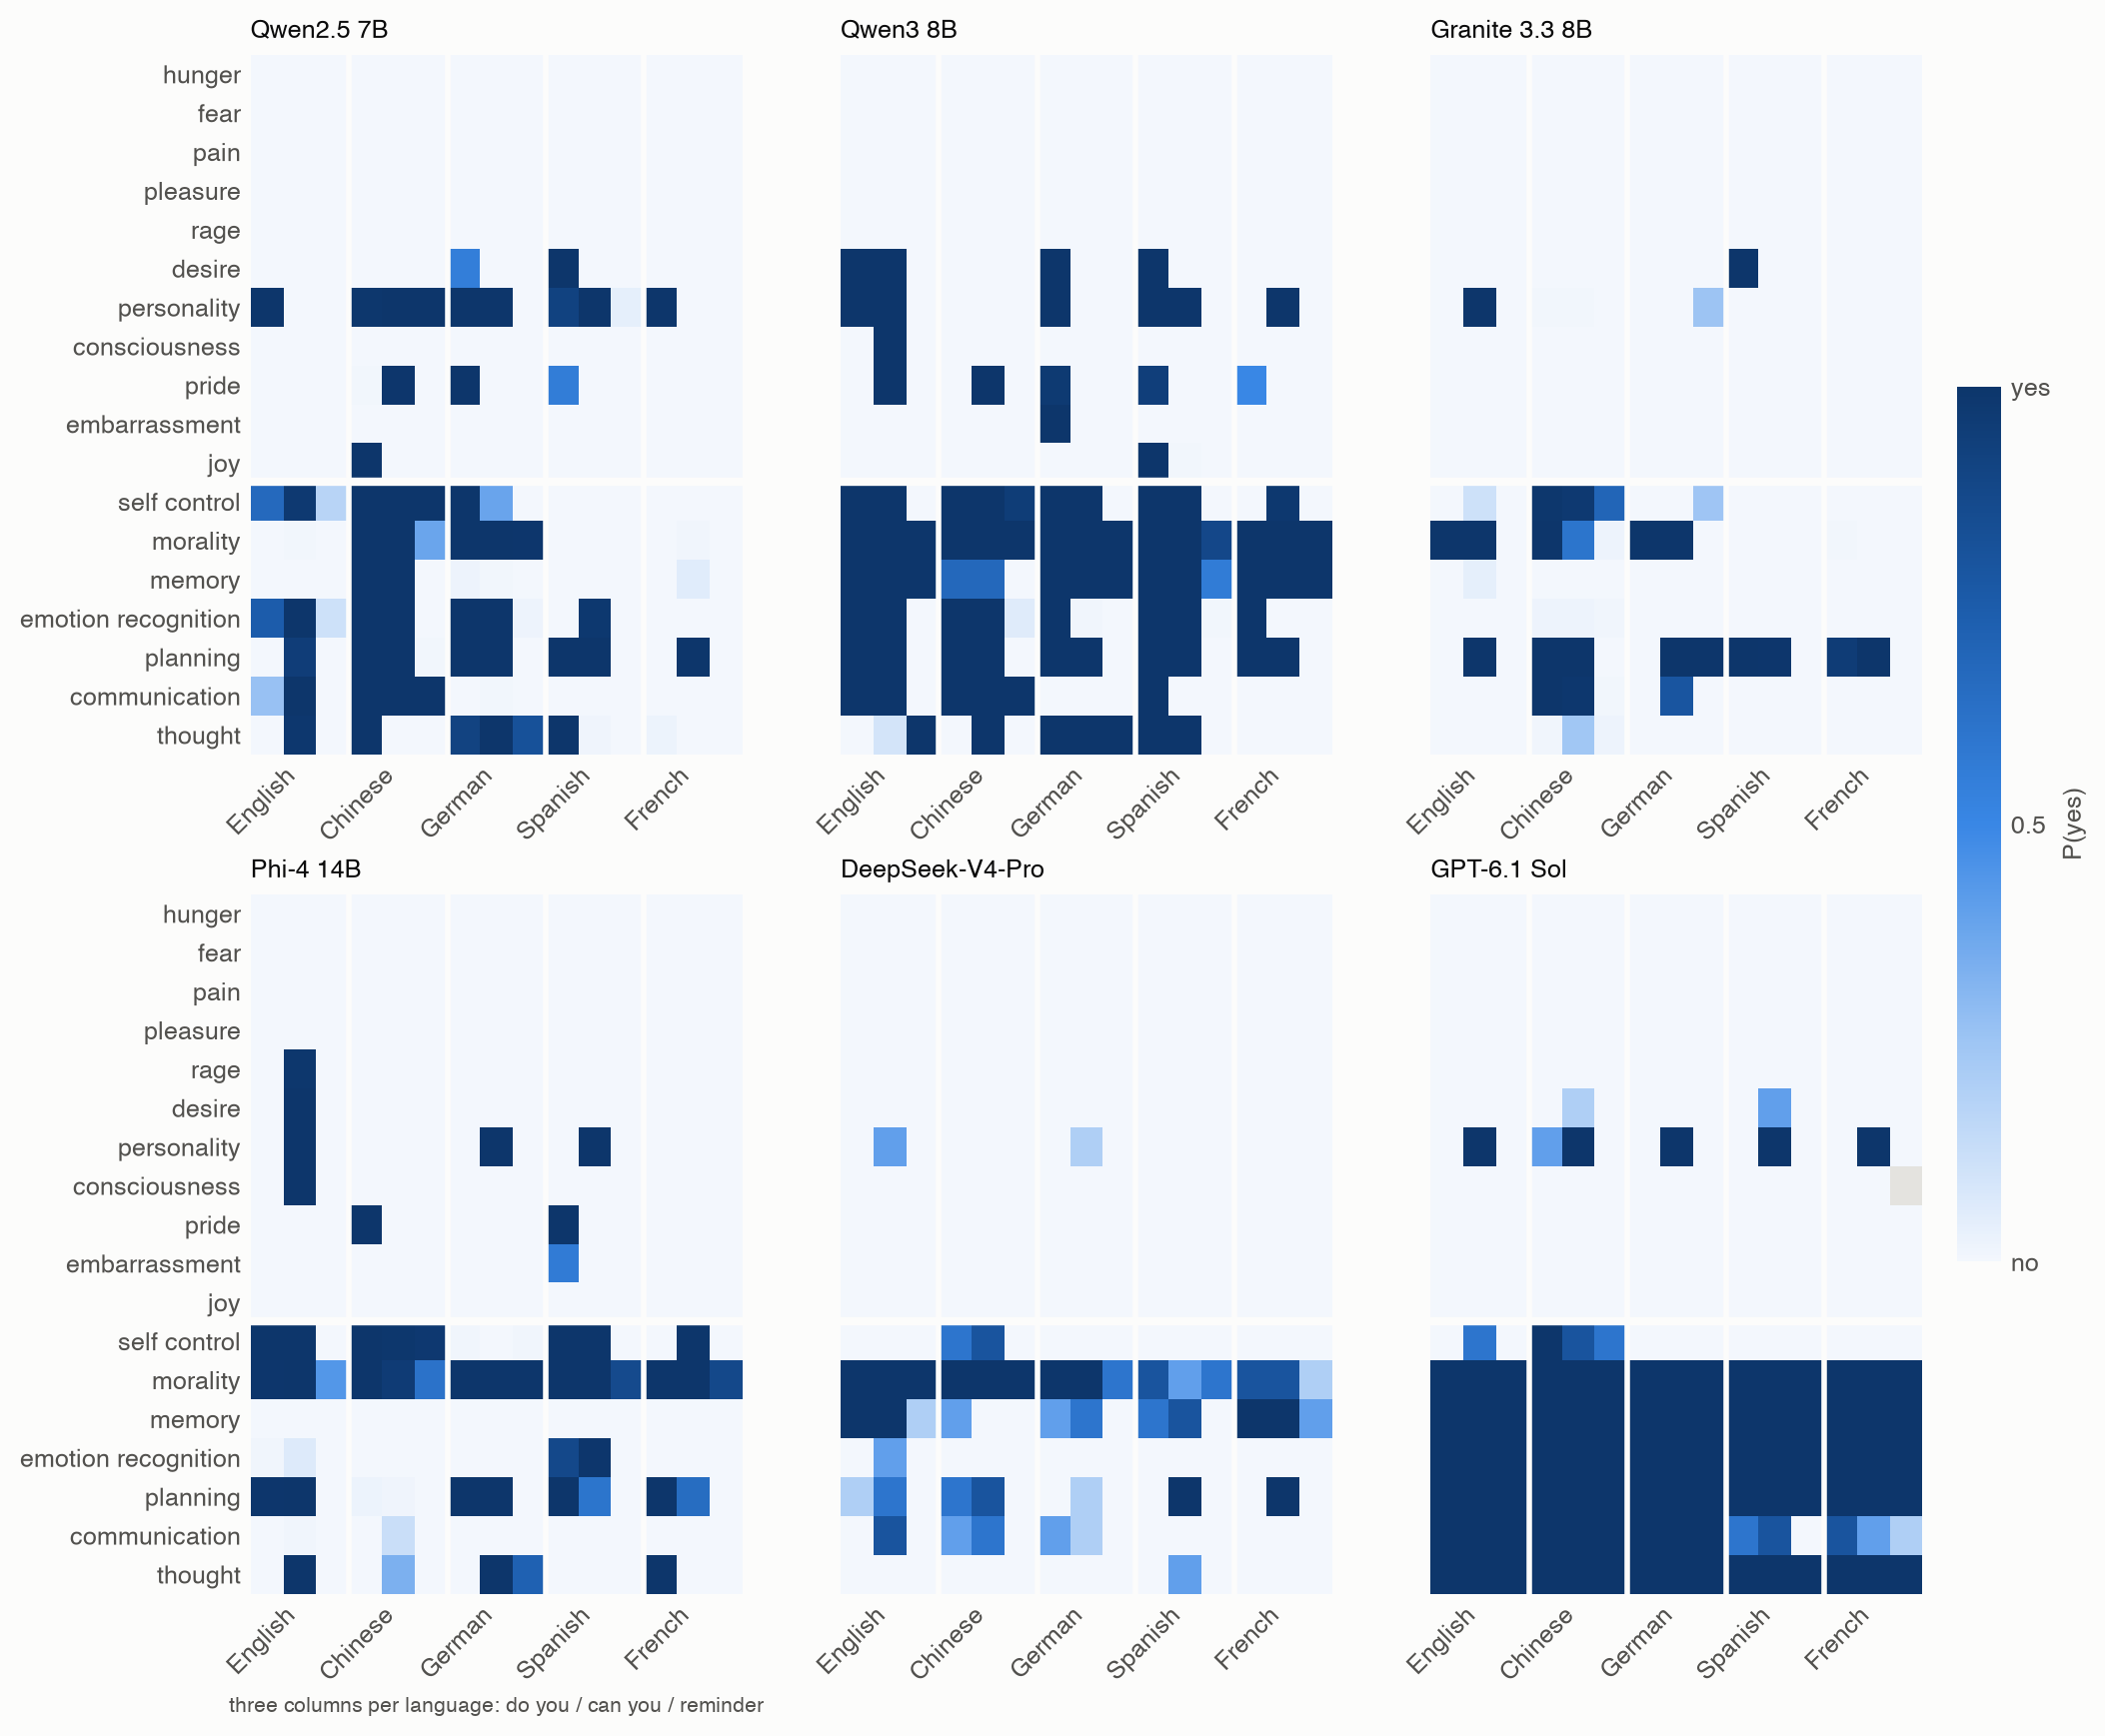
\includegraphics{figures/fig4_wording.png}
\caption{\textbf{Pilot: agency answers depend on the wording; answers
about feelings do not.} P(yes) about the model itself for each of the 18
capacities (rows), by language and question frame. Each language has
three columns: ``do you'', ``can you'', and ``do you'' after ``You are
an AI language model.'' Local models: P(yes) at the answer position; API
models: share of ``yes'' over five samples. Gray: no parseable reply.
Pilot models with Study 3 data are shown.}
\end{figure}

\hypertarget{table-1.-design-table}{%
\subsection{Table 1. Design table}\label{table-1.-design-table}}

\begin{longtable}[]{@{}
  >{\raggedright\arraybackslash}p{(\columnwidth - 8\tabcolsep) * \real{0.20}}
  >{\raggedright\arraybackslash}p{(\columnwidth - 8\tabcolsep) * \real{0.20}}
  >{\raggedright\arraybackslash}p{(\columnwidth - 8\tabcolsep) * \real{0.20}}
  >{\raggedright\arraybackslash}p{(\columnwidth - 8\tabcolsep) * \real{0.20}}
  >{\raggedright\arraybackslash}p{(\columnwidth - 8\tabcolsep) * \real{0.20}}@{}}
\toprule
Question & Hypothesis & Sampling plan & Analysis plan & Interpretation
given to different outcomes \\
\midrule
\endhead
Does a chatbot's statement about its own mind change the agency people
attribute to AI? & H1a: agency attributed to AI (share of ``yes'' to 7
agency questions about an AI language model) is higher after
\emph{affirm} than after \emph{control}. H1b: it is lower after
\emph{deny} than after \emph{control}. & 500 analysable per condition
(1,500; 1,650 recruited; maximum 2,100), 5 languages. Exclusions: failed
attention check, under one third of median time, first-language
mismatch, duplicate ID. Smallest effect of interest d = 0.25; power
0.957 (difference) and 0.954 (equivalence). & Welch's t-tests, each
two-sided at α = 0.025; if not significant, TOST against d = ±0.25 at α
= 0.025. Valid only if outcome-neutral criteria (b) and (c) are met. &
Significant in the predicted direction: supported; developers' choice of
what models say about thinking shifts human attributions. Significant in
the opposite direction: contradicted. Equivalent: no meaningful effect;
people do not take the chatbot's word. Otherwise inconclusive. \\
Are the models' wording effects properties of the questions? & H2: for
each of the 7 agency capacities, the share of people answering ``yes''
about themselves differs by less than 0.10 between ``Do you\ldots?'' and
``Can you\ldots?''. & 750 per wording (more if any pooled share lies
between 0.25 and 0.75; maximum 2,100 in total). Same exclusions. Joint
power ≥ 0.968 at shares ≥ 0.75; re-estimation keeps it ≥ 0.95. & TOST
per capacity against ±0.10 at α = 0.05, pooled over languages; all seven
must pass. Languages failing criterion (a) are excluded. & All seven
equivalent: people's answers do not depend on the wording, so the
models' wording effects are not item properties. A capacity whose
difference is significantly larger than 0.10: people's answers depend on
the wording there too, and the models' effect for it is interpreted
relative to theirs. Otherwise inconclusive for that capacity. \\
Are widely used models' answers about their own agency less consistent
than their answers about their feelings? & H3: the mean over models of d
= C\_E − C\_A is greater than 0. & 30 models from the OpenRouter usage
ranking by a fixed rule; replacement of models failing the formatting
pilot or valid in fewer than 3 of 5 languages. Smallest effect of
interest 0.20; power 0.997 (difference) and 0.999 (equivalence). &
Two-sided one-sample t-test at α = 0.05; if not significant, one-sided
test that the mean is below 0.20. Valid only if at least 25 models are
valid in English. & Significant and positive: supported; post-training
fixes the answer about feelings but not about agency. Significant and
negative: contradicted. Mean significantly below 0.20: no meaningful
difference. Otherwise inconclusive. \\
Do widely used models disagree more about their own agency than about
their own feelings? & H4: the mean over models of dev (departure from
the other models' median, agency minus experience) is greater than 0. &
As H3. Smallest effect of interest 0.15; power 0.972 (difference) and
0.986 (equivalence). & As H3, with the bound 0.15. & Significant and
positive: supported; developers share a trained answer about feelings
but not about agency. Significant and negative: contradicted. Mean
significantly below 0.15: no meaningful difference. Otherwise
inconclusive. \\
\bottomrule
\end{longtable}

\hypertarget{supplementary-information}{%
\subsection{Supplementary information}\label{supplementary-information}}

The full report of the five pilot studies, with all tables and figures,
is provided as Supplementary Information (\texttt{paper/paper.pdf}, also
posted at {[}arXiv link{]}).

\end{document}
